\section{二重积分}

\begin{problem}{交换积分次序}{Change-Order-Integration}
    改变下列积分的顺序：
    \begin{enumerate}
        \item $\int_{-1}^{1} \d x \int_{0}^{\sqrt{1-x^2}} f(x, y) \d y$
        \item $\int_{0}^{2} \d x \int_{2x}^{6-x} f(x, y) \d y$
        \item $\int_{0}^{a} \d y \int_{a-\sqrt{a^2-y^2}}^{a+\sqrt{a^2-y^2}} f(x, y) \d x$
        \item $\int_{a}^{b} \d y \int_{y}^{b} f(x, y) \d x$
        \item $\int_{0}^{1} \d x \int_{0}^{x} f(x, y) \d y + \int_{1}^{2} \d x \int_{0}^{2-x} f(x, y) \d y$
        \item $\int_{0}^{1} \d y \int_{1/2}^{1} f(x, y) \d x + \int_{1}^{2} \d y \int_{1/2}^{1/y} f(x, y) \d x$
    \end{enumerate}
\end{problem}

\begin{solution}
    \ansitem{1} 积分区域为 $x^2 + y^2 \le 1$ 且 $y \ge 0$ 的上半圆盘．

    \begin{center}
        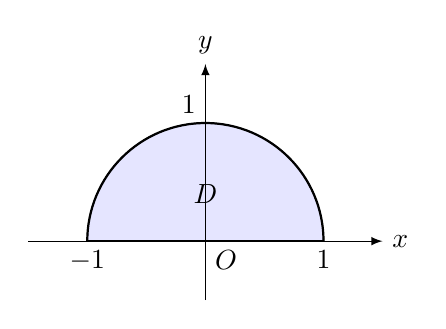
\begin{tikzpicture}[scale=1.5]
            \draw[fill=blue!10] (1,0) arc (0:180:1) -- cycle;
            \draw[-latex] (-1.5,0) -- (1.5,0) node[right] {$x$};
            \draw[-latex] (0,-0.5) -- (0,1.5) node[above] {$y$};
            \draw[thick] (1,0) arc (0:180:1);
            \draw[thick] (-1,0) -- (1,0);
            \node[below] at (1,0) {$1$};
            \node[below] at (-1,0) {$-1$};
            \node[below right] at (0,0) {$O$};
            \node[above left] at (0,1) {$1$};
            \node at (0, 0.4) {$D$};
        \end{tikzpicture}
    \end{center}

    当交换积分次序为先对 $x$ 积分时，$y$ 的取值范围为 $[0, 1]$．对于固定的 $y$，变量 $x$ 从 $-\sqrt{1-y^2}$ 变化至 $\sqrt{1-y^2}$．因此有
    \begin{equation}
        \int_{-1}^{1} \d x \int_{0}^{\sqrt{1-x^2}} f(x, y) \d y = \boxed{\int_{0}^{1} \d y \int_{-\sqrt{1-y^2}}^{\sqrt{1-y^2}} f(x, y) \d x}
    \end{equation}

    \ansitem{2} 积分区域是由直线 $x = 0$、$y = 2x$ 及 $y = 6 - x$ 围成的三角形区域．

    \begin{center}
        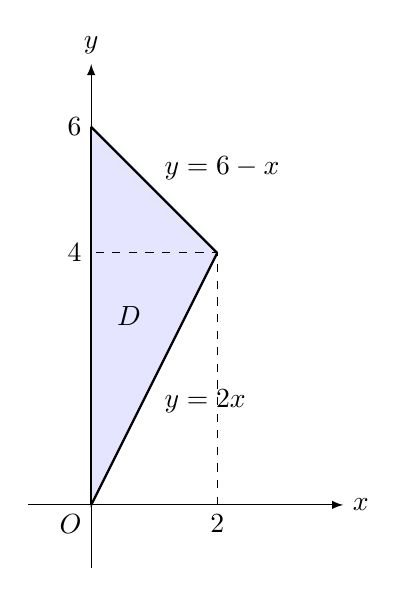
\begin{tikzpicture}[scale=0.8]
            \draw[fill=blue!10] (0,0) -- (2,4) -- (0,6) -- cycle;
            \draw[-latex] (-1,0) -- (4,0) node[right] {$x$};
            \draw[-latex] (0,-1) -- (0,7) node[above] {$y$};
            \draw[thick] (0,0) -- (2,4) node[midway, below right] {$y=2x$};
            \draw[thick] (2,4) -- (0,6) node[midway, above right] {$y=6-x$};
            \draw[thick] (0,0) -- (0,6);
            \draw[dashed] (2,0) node[below] {$2$} -- (2,4) -- (0,4) node[left] {$4$};
            \node[left] at (0,6) {$6$};
            \node[below left] at (0,0) {$O$};
            \node at (0.6, 3) {$D$};
        \end{tikzpicture}
    \end{center}

    其顶点分别为 $(0, 0)$、$(2, 4)$ 及 $(0, 6)$．改变积分次序时需按 $y = 4$ 分段．当 $y \in [0, 4]$ 时，$0 \le x \le \frac{y}{2}$；当 $y \in [4, 6]$ 时，$0 \le x \le 6 - y$．因此有
    \begin{equation}
        \int_{0}^{2} \d x \int_{2x}^{6-x} f(x, y) \d y = \boxed{\int_{0}^{4} \d y \int_{0}^{y/2} f(x, y) \d x + \int_{4}^{6} \d y \int_{0}^{6-y} f(x, y) \d x}
    \end{equation}

    \ansitem{3} 积分区域为圆 $(x-a)^2 + y^2 \le a^2$ 位于 $y \ge 0$ 的上半圆部分．

    \begin{center}
        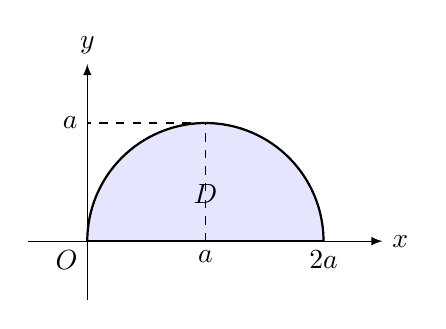
\begin{tikzpicture}[scale=1.5]
            \draw[fill=blue!10] (2,0) arc (0:180:1) -- cycle;
            \draw[-latex] (-0.5,0) -- (2.5,0) node[right] {$x$};
            \draw[-latex] (0,-0.5) -- (0,1.5) node[above] {$y$};
            \draw[thick] (2,0) arc (0:180:1);
            \draw[thick] (0,0) -- (2,0);
            \node[below] at (1,0) {$a$};
            \node[below] at (2,0) {$2a$};
            \node[left] at (0,1) {$a$};
            \draw[dashed] (1,0) -- (1,1) -- (0,1);
            \node[below left] at (0,0) {$O$};
            \node at (1, 0.4) {$D$};
        \end{tikzpicture}
    \end{center}

    由 $x = a \pm \sqrt{a^2 - y^2}$ 可知，圆心在 $(a, 0)$，半径为 $a$．当改变次序先对 $y$ 积分时，$x$ 的范围为 $[0, 2a]$．对于固定的 $x$，有 $0 \le y \le \sqrt{a^2 - (x-a)^2} = \sqrt{2ax - x^2}$．故
    \begin{equation}
        \int_{0}^{a} \d y \int_{a-\sqrt{a^2-y^2}}^{a+\sqrt{a^2-y^2}} f(x, y) \d x = \boxed{\int_{0}^{2a} \d x \int_{0}^{\sqrt{2ax-x^2}} f(x, y) \d y}
    \end{equation}

    \ansitem{4} 积分区域为由直线 $x = y$、$x = b$ 及 $y = a$ 围成的三角形区域．

    \begin{center}
        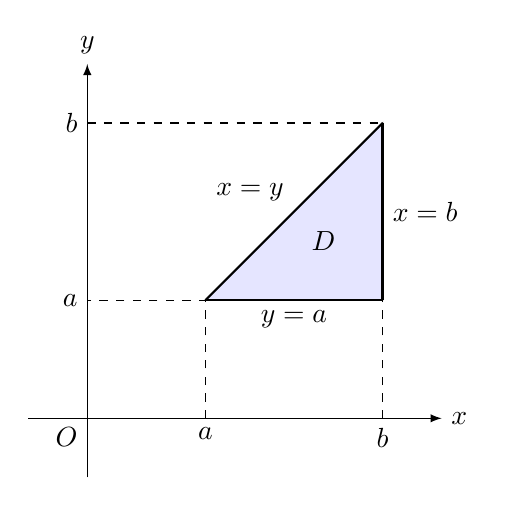
\begin{tikzpicture}[scale=1.5]
            \draw[fill=blue!10] (1,1) -- (2.5,2.5) -- (2.5,1) -- cycle;
            \draw[-latex] (-0.5,0) -- (3,0) node[right] {$x$};
            \draw[-latex] (0,-0.5) -- (0,3) node[above] {$y$};
            \draw[thick] (1,1) -- (2.5,2.5) node[midway, above left] {$x=y$};
            \draw[thick] (2.5,1) -- (2.5,2.5) node[midway, right] {$x=b$};
            \draw[thick] (1,1) -- (2.5,1) node[midway, below] {$y=a$};
            \draw[dashed] (1,0) node[below] {$a$} -- (1,1) -- (0,1) node[left] {$a$};
            \draw[dashed] (2.5,0) node[below] {$b$} -- (2.5,1);
            \draw[dashed] (0,2.5) node[left] {$b$} -- (2.5,2.5);
            \node[below left] at (0,0) {$O$};
            \node at (2, 1.5) {$D$};
        \end{tikzpicture}
    \end{center}

    其顶点为 $(a, a)$、$(b, b)$ 及 $(b, a)$．改为先对 $y$ 积分，则 $x$ 范围为 $[a, b]$．对于固定的 $x$，$y$ 的范围由下边界 $y = a$ 至上边界 $y = x$．即
    \begin{equation}
        \int_{a}^{b} \d y \int_{y}^{b} f(x, y) \d x = \boxed{\int_{a}^{b} \d x \int_{a}^{x} f(x, y) \d y}
    \end{equation}

    \ansitem{5} 积分区域由两个三角形区域合并而成．

    \begin{center}
        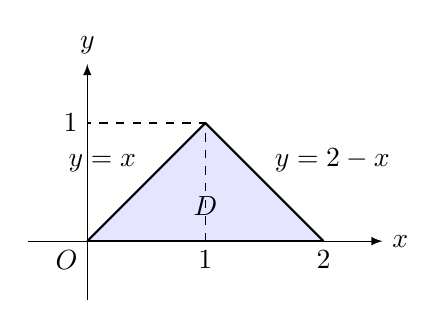
\begin{tikzpicture}[scale=1.5]
            \draw[fill=blue!10] (0,0) -- (1,1) -- (2,0) -- cycle;
            \draw[-latex] (-0.5,0) -- (2.5,0) node[right] {$x$};
            \draw[-latex] (0,-0.5) -- (0,1.5) node[above] {$y$};
            \draw[thick] (0,0) -- (1,1) node[midway, above left] {$y=x$};
            \draw[thick] (1,1) -- (2,0) node[midway, above right] {$y=2-x$};
            \draw[thick] (0,0) -- (2,0);
            \draw[dashed] (1,0) node[below] {$1$} -- (1,1) -- (0,1) node[left] {$1$};
            \node[below] at (2,0) {$2$};
            \node[below left] at (0,0) {$O$};
            \node at (1, 0.3) {$D$};
        \end{tikzpicture}
    \end{center}

    合并后的区域是以 $(0, 0)$、$(1, 1)$、$(2, 0)$ 为顶点的三角形．若改为先对 $x$ 积分，则 $y$ 的范围为 $[0, 1]$．对于固定的 $y$，$x$ 从直线 $x = y$ 变化到 $x = 2 - y$．故有
    \begin{equation}
        \int_{0}^{1} \d x \int_{0}^{x} f(x, y) \d y + \int_{1}^{2} \d x \int_{0}^{2-x} f(x, y) \d y = \boxed{\int_{0}^{1} \d y \int_{y}^{2-y} f(x, y) \d x}
    \end{equation}

    \ansitem{6} 积分区域由矩形区域与曲边梯形区域合并而成．

    \begin{center}
        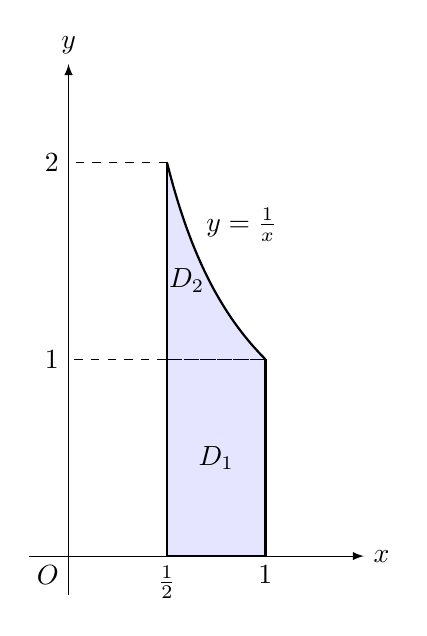
\begin{tikzpicture}[scale=2.5]
            % 填充区域（在 plot 前添加 -- 确保路径闭合无断裂，并增加 samples 使曲线平滑）
            \fill[blue!10] (0.5,0) -- (1,0) -- (1,1) -- plot[domain=1:0.5, samples=50] (\x, {1/\x}) -- (0.5,2) -- cycle;

            % 坐标轴
            \draw[-latex] (-0.2,0) -- (1.5,0) node[right] {$x$};
            \draw[-latex] (0,-0.2) -- (0,2.5) node[above] {$y$};

            % 区域边界
            \draw[thick] (0.5,0) -- (1,0);
            \draw[thick] (1,0) -- (1,1);
            \draw[thick] plot[domain=1:0.5, samples=50] (\x, {1/\x});
            \draw[thick] (0.5,0) -- (0.5,2);

            % 辅助线与坐标刻度
            \draw[dashed] (0.5,2) -- (0,2) node[left] {$2$};
            \draw[dashed] (1,1) -- (0,1) node[left] {$1$};
            \draw[dashed] (0.5,1) -- (1,1); % 标示原积分的两部分区域分界线

            \node[below] at (0.5,0) {$\frac{1}{2}$};
            \node[below] at (1,0) {$1$};
            \node[above right] at (0.65, 1.55) {$y=\frac{1}{x}$};
            \node[below left] at (0,0) {$O$};

            % 区域标注（对应原式的两部分积分）
            \node at (0.75, 0.5) {$D_1$};
            \node at (0.6, 1.4) {$D_2$};
        \end{tikzpicture}
    \end{center}

    第一部分区域为 $x \in [1/2, 1]$、$y \in [0, 1]$；第二部分由 $y \in [1, 2]$ 且 $1/2 \le x \le 1/y$ 限定．合并后的总区域满足 $1/2 \le x \le 1$．对于固定的 $x$，变量 $y$ 的范围从 $0$ 到曲线 $y = 1/x$．因此
    \begin{equation}
        \int_{0}^{1} \d y \int_{1/2}^{1} f(x, y) \d x + \int_{1}^{2} \d y \int_{1/2}^{1/y} f(x, y) \d x = \boxed{\int_{1/2}^{1} \d x \int_{0}^{1/x} f(x, y) \d y}
    \end{equation}
\end{solution}


\begin{problem}{二重积分计算}{}
    计算下列积分：
    \begin{enumerate}
        \item $\iint_{D} \frac{y}{\left(1+x^{2}+y^{2}\right)^{3 / 2}} \d x \d y, D=[0,1] \times [0,1]$；
        \item $\iint_{D} \sin (x+y) \d x \d y, D=[0, \uppi] \times [0,\uppi]$；
        \item $\iint_{D} \cos (x+y) \d x \d y, D$：由 $y=\uppi, x=y, x=0$ 围成；
        \item $\iint_{D}(x+y) \d x \d y, D$：由 $x^{2}+y^{2}=a^{2}$ 围成的圆在第一象限部分；
        \item $\iint_{D}(x+y-1) \d x \d y, D$：由 $y=x, y=x+a, y=a, y=3 a$ 围成；
        \item $\iint_{D} \frac{\sin y}{y} \d x \d y, D$：由 $y=x$ 和 $x=y^{2}$ 围成；
        \item $\iint_{D} \frac{x^{2}}{y^{2}} \d x \d y, D$：由 $x=2, y=x$ 及 $x y=1$ 围成；
        \item $\iint_{D}|\cos (x+y)| \d x \d y$，$D$：由 $y=x, y=0, x=\frac{\uppi}{2}$ 所围成．
    \end{enumerate}
\end{problem}

\begin{solution}
    \ansitem{1}

    根据累次积分的计算方法，有
    \begin{equation}
        \begin{aligned}
            \iint_{D} \frac{y}{\left(1+x^{2}+y^{2}\right)^{3 / 2}} \d x \d y & = \int_{0}^{1} \d x \int_{0}^{1} \frac{y}{\left(1+x^{2}+y^{2}\right)^{3 / 2}} \d y                     \\
                                                                             & = \int_{0}^{1} \left[ -\frac{1}{\sqrt{1+x^{2}+y^{2}}} \right]_{0}^{1} \d x                             \\
                                                                             & = \int_{0}^{1} \left( \frac{1}{\sqrt{1+x^{2}}} - \frac{1}{\sqrt{x^{2}+2}} \right) \d x                 \\
                                                                             & = \left[ \ln \left( x + \sqrt{1+x^{2}} \right) - \ln \left( x + \sqrt{2+x^{2}} \right) \right]_{0}^{1} \\
                                                                             & = \ln (1+\sqrt{2}) - \ln (1+\sqrt{3}) + \ln \sqrt{2}
        \end{aligned}
    \end{equation}
    整理得到
    \begin{equation}
        I = \boxed{\ln \frac{2+\sqrt{2}}{1+\sqrt{3}}}
    \end{equation}

    \ansitem{2}

    积分区域为矩形区域，直接计算
    \begin{equation}
        \begin{aligned}
            \iint_{D} \sin (x+y) \d x \d y & = \int_{0}^{\uppi} \d x \int_{0}^{\uppi} \sin (x+y) \d y \\
                                           & = \int_{0}^{\uppi} [-\cos (x+y)]_{0}^{\uppi} \d x        \\
                                           & = \int_{0}^{\uppi} (\cos x - \cos (x+\uppi)) \d x        \\
                                           & = \int_{0}^{\uppi} 2 \cos x \d x
        \end{aligned}
    \end{equation}
    于是有
    \begin{equation}
        I = \boxed{0}
    \end{equation}

    \ansitem{3}

    积分区域为 $D = \{ (x, y) \mid 0 \le y \le \uppi, 0 \le x \le y \}$，则
    \begin{equation}
        \begin{aligned}
            \iint_{D} \cos (x+y) \d x \d y & = \int_{0}^{\uppi} \d y \int_{0}^{y} \cos (x+y) \d x                \\
                                           & = \int_{0}^{\uppi} [\sin(x+y)]_{0}^{y} \d y                         \\
                                           & = \int_{0}^{\uppi} (\sin 2y - \sin y) \d y                          \\
                                           & = \left[ -\frac{1}{2} \cos 2y + \cos y \right]_{0}^{\uppi}          \\
                                           & = \left( -\frac{1}{2} - 1 \right) - \left( -\frac{1}{2} + 1 \right)
        \end{aligned}
    \end{equation}
    计算得出
    \begin{equation}
        I = \boxed{-2}
    \end{equation}

    \ansitem{4}

    利用极坐标变换，令 $x = r \cos \theta$、$y = r \sin \theta$，其雅可比行列式为 $r$，积分区域变为 $D' = \{ (r, \theta) \mid 0 \le \theta \le \frac{\uppi}{2}, 0 \le r \le a \}$
    \begin{equation}
        \begin{aligned}
            \iint_{D} (x+y) \d x \d y & = \int_{0}^{\uppi/2} \d \theta \int_{0}^{a} r (\cos \theta + \sin \theta) r \d r           \\
                                      & = \int_{0}^{\uppi/2} (\cos \theta + \sin \theta) \d \theta \int_{0}^{a} r^{2} \d r         \\
                                      & = [\sin \theta - \cos \theta]_{0}^{\uppi/2} \cdot \left[ \frac{1}{3} r^{3} \right]_{0}^{a} \\
                                      & = (1 - (-1)) \cdot \frac{a^{3}}{3}
        \end{aligned}
    \end{equation}
    因此
    \begin{equation}
        I = \boxed{\frac{2 a^{3}}{3}}
    \end{equation}

    \ansitem{5}

    作变量替换 $u = y-x$、$v = y$，变换的雅可比行列式绝对值为 $1$，区域 $D$ 映射为矩形区域 $0 \le u \le a$、$a \le v \le 3a$
    \begin{equation}
        \begin{aligned}
            \iint_{D} (x+y-1) \d x \d y & = \int_{a}^{3 a} \d v \int_{0}^{a} (2 v - u - 1) \d u                       \\
                                        & = \int_{a}^{3 a} \left[ 2 u v - \frac{1}{2} u^{2} - u \right]_{0}^{a} \d v  \\
                                        & = \int_{a}^{3 a} (2 a v - \frac{1}{2} a^{2} - a) \d v                       \\
                                        & = \left[ a v^{2} - \left( \frac{1}{2} a^{2} + a \right) v \right]_{a}^{3 a} \\
                                        & = 8 a^{3} - \left( \frac{1}{2} a^{2} + a \right) (2 a)
        \end{aligned}
    \end{equation}
    化简得到
    \begin{equation}
        I = \boxed{7 a^{3}-2 a^{2}}
    \end{equation}

    \ansitem{6}

    积分区域为 $D = \{ (x, y) \mid 0 \le y \le 1, y^{2} \le x \le y \}$，采用先 $x$ 后 $y$ 的积分次序
    \begin{equation}
        \begin{aligned}
            \iint_{D} \frac{\sin y}{y} \d x \d y & = \int_{0}^{1} \frac{\sin y}{y} \d y \int_{y^{2}}^{y} \d x \\
                                                 & = \int_{0}^{1} \frac{\sin y}{y} (y - y^{2}) \d y           \\
                                                 & = \int_{0}^{1} (\sin y - y \sin y) \d y                    \\
                                                 & = [-\cos y]_{0}^{1} - [ -y \cos y + \sin y ]_{0}^{1}       \\
                                                 & = (1 - \cos 1) - (- \cos 1 + \sin 1)
        \end{aligned}
    \end{equation}
    得到
    \begin{equation}
        I = \boxed{1-\sin 1}
    \end{equation}

    \ansitem{7}

    积分区域 $D$ 的范围为 $1 \le x \le 2$、$\frac{1}{x} \le y \le x$，则
    \begin{equation}
        \begin{aligned}
            \iint_{D} \frac{x^{2}}{y^{2}} \d x \d y & = \int_{1}^{2} x^{2} \d x \int_{1 / x}^{x} \frac{1}{y^{2}} \d y   \\
                                                    & = \int_{1}^{2} x^{2} \left[ -\frac{1}{y} \right]_{1 / x}^{x} \d x \\
                                                    & = \int_{1}^{2} x^{2} \left( x - \frac{1}{x} \right) \d x          \\
                                                    & = \left[ \frac{1}{4} x^{4} - \frac{1}{2} x^{2} \right]_{1}^{2}
        \end{aligned}
    \end{equation}
    计算结果为
    \begin{equation}
        I = \boxed{\frac{9}{4}}
    \end{equation}

    \ansitem{8}

    积分区域为 $D = \{ (x, y) \mid 0 \le x \le \frac{\uppi}{2}, 0 \le y \le x \}$．直线 $x+y = \frac{\uppi}{2}$ 将区域分为两部分，分别对应 $\cos(x+y)$ 的正负性
    \begin{equation}
        \begin{aligned}
            I & = \iint_{D_{x+y \le \frac{\uppi}{2}}} \cos (x+y) \d A + \iint_{D_{x+y \ge \frac{\uppi}{2}}} -\cos (x+y) \d A                         \\
              & = \int_{0}^{\uppi/4} \d y \int_{y}^{\uppi/2-y} \cos (x+y) \d x + \int_{\uppi/4}^{\uppi/2} \d x \int_{\uppi/2-x}^{x} -\cos (x+y) \d y \\
              & = \int_{0}^{\uppi/4} (1 - \sin 2y) \d y + \int_{\uppi/4}^{\uppi/2} (1 - \sin 2x) \d x                                                \\
              & = \left[ y + \frac{1}{2} \cos 2y \right]_{0}^{\uppi/4} + \left[ x + \frac{1}{2} \cos 2x \right]_{\uppi/4}^{\uppi/2}
        \end{aligned}
    \end{equation}
    计算得出
    \begin{equation}
        I = \left( \frac{\uppi}{4} - \frac{1}{2} \right) + \left( \frac{\uppi}{4} - \frac{1}{2} \right) = \boxed{\frac{\uppi}{2}-1}
    \end{equation}
\end{solution}


\begin{problem}{利用对称性计算二重积分}{Double-Integral-Symmetry}
    利用函数的奇偶性计算下列积分：
    \begin{enumerate}
        \item $\iint_{D} (x^{2}+y^{2}) \d x \d y$，$D: -1 \le x \le 1, -1 \le y \le 1$；
        \item $\iint_{D} \sin x \sin y \d x \d y$，$D: x^{2}-y^{2}=1, x^{2}+y^{2}=9$ 围成的含原点的部分；
    \end{enumerate}
\end{problem}

\begin{solution}
    \ansitem{1}

    由于积分区域 $D = [-1, 1] \times [-1, 1]$ 关于 $x$ 轴与 $y$ 轴均具有对称性，且被积函数 $f(x, y) = x^2 + y^2$ 为偶函数，由二重积分的对称性可知
    \begin{equation}\label{eq:calc-1}
        \begin{aligned}
            \iint_{D} (x^2 + y^2) \d x \d y & = \int_{-1}^1 \d y \int_{-1}^1 (x^2 + y^2) \d x                       \\
                                            & = \int_{-1}^1 \left[ \frac{1}{3}x^3 + y^2 x \right]_{x=-1}^{x=1} \d y \\
                                            & = \int_{-1}^1 \left( \frac{2}{3} + 2y^2 \right) \d y.
        \end{aligned}
    \end{equation}
    进一步计算 \zcref{eq:calc-1} 中的定积分，可得
    \begin{equation}
        \iint_{D} (x^2 + y^2) \d x \d y = \left[ \frac{2}{3}y + \frac{2}{3}y^3 \right]_{-1}^1 = \frac{4}{3} - \left( -\frac{4}{3} \right) = \frac{8}{3}.
    \end{equation}
    最终计算结果为
    \begin{equation}
        \boxed{\iint_{D} (x^2 + y^2) \d x \d y = \frac{8}{3}}
    \end{equation}

    \ansitem{2}

    观察积分区域 $D$ 的边界方程 $x^2 - y^2 = 1$ 与 $x^2 + y^2 = 9$ 可知，若点 $(x, y) \in D$，则点 $(-x, y) \in D$．这意味着区域 $D$ 关于 $y$ 轴（即直线 $x=0$）是对称的．
    令被积函数为 $g(x, y) = \sin x \sin y$，考察其关于变量 $x$ 的奇偶性
    \begin{equation}\label{eq:parity-check}
        g(-x, y) = \sin(-x) \sin y = -\sin x \sin y = -g(x, y).
    \end{equation}
    由 \zcref{eq:parity-check} 可知，$g(x, y)$ 是关于 $x$ 的奇函数．根据二重积分的对称性质，奇函数在关于坐标轴对称的区域上的积分为零．故有
    \begin{equation}
        \boxed{\iint_{D} \sin x \sin y \d x \d y = 0}
    \end{equation}
\end{solution}


\begin{problem}{可积函数乘积的积分}{Integrability-Product}
    设函数 $\varphi$ 和 $\psi$ 分别在区间 $[a, b]$ 和 $[c, d]$ 上可积，求证 $f(x, y) = \varphi(x) \psi(y)$ 在 $D = [a, b] \times [c, d]$ 上可积，且有
    \begin{equation}
        \iint_{D} f(x, y) \d x \d y = \int_{a}^{b} \varphi(x) \d x \int_{c}^{d} \psi(x) \d x.
    \end{equation}
\end{problem}

\begin{myproof}

    由于 $\varphi(x)$ 与 $\psi(y)$ 分别在闭区间上可积，故它们在该区间上必有界．设存在常数 $M_1, M_2 > 0$ 使得 $|\varphi(x)| \le M_1$ 且 $|\psi(y)| \le M_2$，则有
    \begin{equation}
        |f(x, y)| = |\varphi(x)| \cdot |\psi(y)| \le M_1 M_2,
    \end{equation}
    即 $f(x, y)$ 在矩形区域 $D$ 上有界．记 $S_\varphi$ 与 $S_\psi$ 分别为 $\varphi$ 与 $\psi$ 的不连续点集，由可积性定义可知其勒贝格测度 $\mu(S_\varphi) = 0$ 且 $\mu(S_\psi) = 0$．函数 $f(x, y)$ 的不连续点集 $S_f$ 满足
    \begin{equation}
        S_f \subseteq (S_\varphi \times [c, d]) \cup ([a, b] \times S_\psi).
    \end{equation}
    根据测度性质，零测集与有界闭区间的笛卡尔积仍为零测集，故 $\mu(S_f) = 0$．因此 $f(x, y)$ 在 $D$ 上可积．
    根据累次积分定理（Fubini 定理），可得
    \begin{equation}\label{eq:fubini-calc}
        \iint_{D} f(x, y) \d x \d y = \int_{a}^{b} \left( \int_{c}^{d} \varphi(x) \psi(y) \d y \right) \d x.
    \end{equation}
    在内层关于 $y$ 的积分中，$\varphi(x)$ 视为常数，可移至积分号外
    \begin{equation}
        \iint_{D} f(x, y) \d x \d y = \int_{a}^{b} \varphi(x) \left( \int_{c}^{d} \psi(y) \d y \right) \d x.
    \end{equation}
    由于 $\int_{c}^{d} \psi(y) \d y$ 是一个确定的常数，将其移至外层积分号外，并将积分变量 $y$ 重新记为 $x$（作为哑变量），即证得
    \begin{equation}
        \boxed{\iint_{D} f(x, y) \d x \d y = \int_{a}^{b} \varphi(x) \d x \int_{c}^{d} \psi(x) \d x}
    \end{equation}
\end{myproof}


\begin{problem}{定积分恒等式}{Integral-Identities}
    设函数 $f(x)$ 在 $[0, a]$ 上连续，证明：
    \begin{enumerate}
        \item $\int_0^a \d x \int_0^x f(x)f(y) \d y = \frac{1}{2} \left( \int_0^a f(x) \d x \right)^2$；
        \item $\int_0^a \d x \int_0^x f(y) \d y = \int_0^a (a-x)f(x) \d x$．
    \end{enumerate}
\end{problem}

\begin{myproof}
    \ansitem{1}

    记该二重积分为 $I$．由于积分区域为三角形区域 $D = \{ (x, y) \mid 0 \le x \le a, 0 \le y \le x \}$，交换积分次序可得
    \begin{equation}
        I = \int_0^a \d y \int_y^a f(x)f(y) \d x \label{eq:Ident-1}
    \end{equation}
    利用变量的对等性，将 \zcref{eq:Ident-1} 中的 $x$ 与 $y$ 互换，有
    \begin{equation}
        I = \int_0^a \d x \int_x^a f(y)f(x) \d y \label{eq:Ident-2}
    \end{equation}
    将原式与 \zcref{eq:Ident-2} 相加，得
    \begin{equation}
        \begin{aligned}
            2I & = \int_0^a \d x \int_0^x f(x)f(y) \d y + \int_0^a \d x \int_x^a f(x)f(y) \d y \\
               & = \int_0^a f(x) \left[ \int_0^x f(y) \d y + \int_x^a f(y) \d y \right] \d x   \\
               & = \int_0^a f(x) \left[ \int_0^a f(y) \d y \right] \d x                        \\
               & = \left( \int_0^a f(x) \d x \right) \left( \int_0^a f(y) \d y \right)         \\
               & = \left( \int_0^a f(x) \d x \right)^2
        \end{aligned}
    \end{equation}
    故有
    \begin{equation}
        I = \frac{1}{2} \left( \int_0^a f(x) \d x \right)^2
    \end{equation}

    \ansitem{2}

    考虑积分区域 $D = \{ (x, y) \mid 0 \le x \le a, 0 \le y \le x \}$，交换积分次序可得
    \begin{equation}
        \int_0^a \d x \int_0^x f(y) \d y = \int_0^a \d y \int_y^a f(y) \d x
    \end{equation}
    计算内部关于 $x$ 的定积分
    \begin{equation}
        \int_y^a f(y) \d x = f(y) \int_y^a \d x = (a - y)f(y)
    \end{equation}
    于是有
    \begin{equation}
        \int_0^a \d y \int_y^a f(y) \d x = \int_0^a (a - y)f(y) \d y
    \end{equation}
    将积分变量 $y$ 替换为 $x$，即证得
    \begin{equation}
        \int_0^a \d x \int_0^x f(y) \d y = \int_0^a (a - x)f(x) \d x
    \end{equation}
\end{myproof}


\begin{problem}{偏导数重积分}{Partial-Derivative-Integral}
    设函数 $f(x, y)$ 有连续的二阶偏导数，在 $D = [a, b] \times [c, d]$ 上，求积分
    \begin{equation}
        \iint_D \frac{\partial^2 f(x, y)}{\partial x \partial y} \d x \d y
    \end{equation}
\end{problem}

\begin{solution}
    根据累次积分计算规则，有
    \begin{equation}
        \iint_D \frac{\partial^2 f(x, y)}{\partial x \partial y} \d x \d y = \int_c^d \d y \int_a^b \frac{\partial}{\partial x} \left( \frac{\partial f(x, y)}{\partial y} \right) \d x
    \end{equation}
    根据微积分基本定理计算内部积分
    \begin{equation}
        \int_a^b \frac{\partial}{\partial x} \left( \frac{\partial f(x, y)}{\partial y} \right) \d x = \left. \frac{\partial f(x, y)}{\partial y} \right|_{x=a}^{x=b} = \frac{\partial f(b, y)}{\partial y} - \frac{\partial f(a, y)}{\partial y}
    \end{equation}
    代回原式继续积分
    \begin{equation}
        \begin{aligned}
            \int_c^d \left( \frac{\partial f(b, y)}{\partial y} - \frac{\partial f(a, y)}{\partial y} \right) \d y & = \int_c^d \frac{\partial f(b, y)}{\partial y} \d y - \int_c^d \frac{\partial f(a, y)}{\partial y} \d y \\
                                                                                                                   & = [f(b, d) - f(b, c)] - [f(a, d) - f(a, c)]
        \end{aligned}
    \end{equation}
    整理合并项得
    \begin{equation}
        \iint_D \frac{\partial^2 f(x, y)}{\partial x \partial y} \d x \d y = \boxed{f(b, d) - f(b, c) - f(a, d) + f(a, c)}
    \end{equation}
\end{solution}


\begin{problem}{二重积分极限}{Double-Integral-Limit}
    设函数 $f(x, y)$ 连续，求极限
    \begin{equation}
        \lim_{r \to 0} \frac{1}{\uppi r^2} \iint_{x^2 + y^2 \le r^2} f(x, y) \d x \d y
    \end{equation}
\end{problem}

\begin{solution}
    令 $D_r = \{ (x, y) \mid x^2 + y^2 \le r^2 \}$．根据二重积分中值定理，由于 $f(x, y)$ 在闭区域 $D_r$ 上连续，存在点 $(\xi, \eta) \in D_r$，使得
    \begin{equation}
        \iint_{D_r} f(x, y) \d x \d y = f(\xi, \eta) \cdot \operatorname{Area}(D_r) \label{eq:MVT}
    \end{equation}
    其中区域 $D_r$ 的面积为
    \begin{equation}
        \operatorname{Area}(D_r) = \uppi r^2
    \end{equation}
    将 \zcref{eq:MVT} 代入极限表达式中，得
    \begin{equation}
        \lim_{r \to 0} \frac{1}{\uppi r^2} \cdot f(\xi, \eta) \cdot \uppi r^2 = \lim_{r \to 0} f(\xi, \eta)
    \end{equation}
    当 $r \to 0$ 时，由于 $(\xi, \eta) \in D_r$，显然有 $(\xi, \eta) \to (0, 0)$．由 $f(x, y)$ 的连续性可知
    \begin{equation}
        \lim_{r \to 0} f(\xi, \eta) = f(0, 0)
    \end{equation}
    故最终结果为
    \begin{equation}
        \lim_{r \to 0} \frac{1}{\uppi r^2} \iint_{x^2 + y^2 \le r^2} f(x, y) \d x \d y = \boxed{f(0, 0)}
    \end{equation}
\end{solution}

\endinput
